%
We will now compare non-adversarial performance of the compact frequency estimators (CFEs) by measuring the ability of these structures in identifying the most frequent (heavy) elements of a stream. Finding the heavy elements of a stream is the typical use case of CFEs and as such these structures are used for that purpose in many systems level applications~\cite{yang2019heavykeeper,mandal2018topkapi,radu2010,metwally2006,cormode2005improved,charikar2002finding,manku2002approximate}. The ability to accurately identify these heavy elements is based on a CFE's ability to accurately make frequency estimations on these heavy elements, while maintaining the ability to make accurate frequency estimations on the non-heavy elements, such that one would be able to distinguish between the two classes of elements. Therefore, we experimentally measure the non-adversarial performance of these structure by comparing a number of performance metrics in identifying heavy elements across three different streams. 

\paragraph{Data Streams} We have three different streams we experiment with. We sourced two streams from a frequent item mining dataset repository\footnote{\url{http://fimi.uantwerpen.be/data/}}. We also sourced an additional stream by processing a large English language novel from Project Gutenberg. %\mia{Why are these sets good to test the 'honest' setting behaviour of our CFEs? (we can also comment on the 'goodness' of each separately) Are these the ones used to inspect honest setting behaviour of some other CFEs? If not, why didn't we use the same data-sets as papers inspecting other CFEs?} 

We summarize each of these three streams and why they are of particular interest to experiment on below.

\begin{enumerate}

    \item \textbf{Kosarak Stream:} This data collection contained anonymized click-rate data collected from visits to an online Hungarian news site. The resultant stream is of total length~$8,019,015$ with~$41,270$ distinct elements. As aforementioned, we sourced this stream from a frequent item mining dataset repository which is a collection of data sets meant to test frequent item finding algorithms on -- the very task which we are doing. We flattened the raw collection of data such that it would resemble a stream that could be processed item-by-item.

    \item \textbf{Novel Stream:} We created a stream by processing the individual words sequentially of The Project Gutenberg eBook plaintext edition of the~$1851$ English-language novel \textit{Moby-Dick; or, The Whale} by Herman Melville (ignoring capitalization and non-alphabetical characters)~\cite{melville1851}. %For generality and ease of reference we map all words to their frequency rank in the true stream (i.e. the word `the' maps to `1' and so on). 
    Long bodies of natural language obey an approximate Zipf distribution as the frequency of any word is inversely proportional to its rank in an ordered frequency list~\cite{adamic2002zipf}.  It is of interest to measure compact frequency estimators performance against data following a Zipf distribution~\cite{charikar2002finding,cormode2005s,yang2019heavykeeper,radu2010,metwally2006,manku2002approximate}. The stream is of total length~$2,174,111$ with~$19,215$ distinct elements.
 
    \item \textbf{Retail Stream:} This data collection contained anonymized shopping data from a Belgian retail store. The resultant stream is of total length~$908,576$ and contains~$16,740$ distinct elements. This data set is also from the frequent items mining dataset repository. As with the Kosarak stream we flattened the raw data such that it would resemble a stream after processing. 
\end{enumerate}

\begin{figure*}[!ht]
  \centering
  \minipage{0.32\textwidth}
    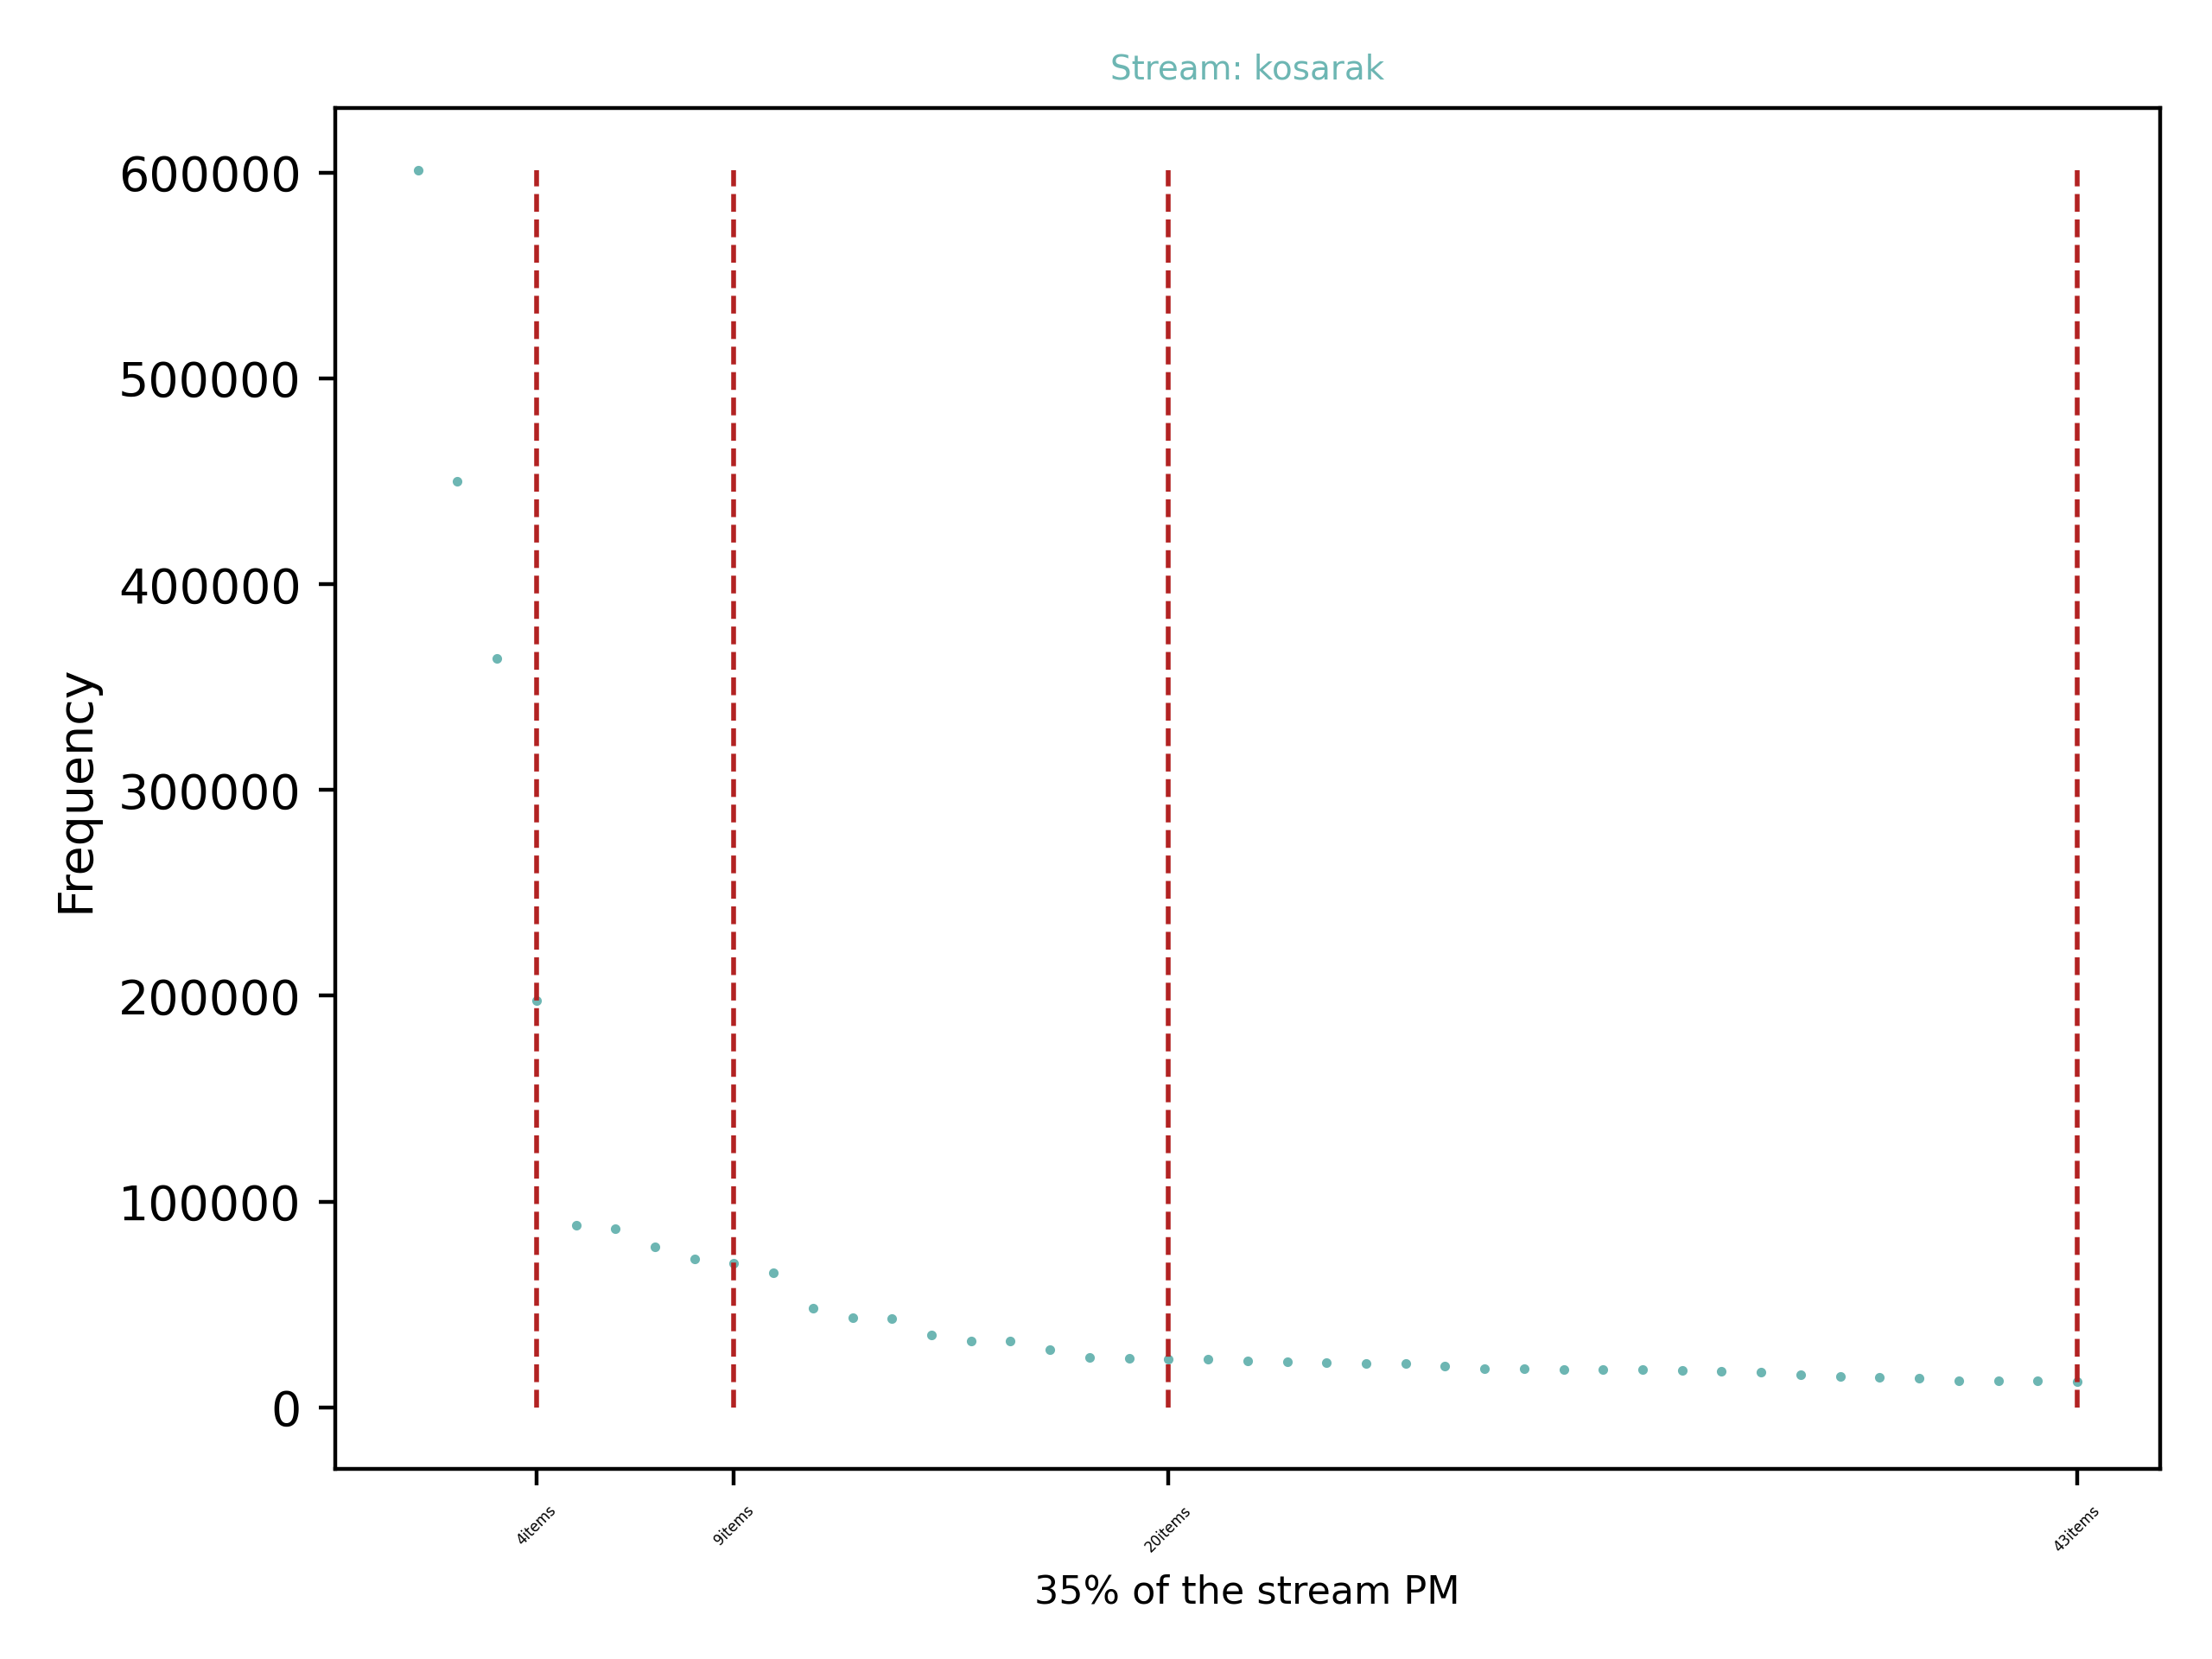
\includegraphics[width=\linewidth]{chapters/ch3_cfe/ch3_images/kosarak_pm.png}
    \caption*{Kosarak stream}
  \endminipage\hfill
  \minipage{0.32\textwidth}
    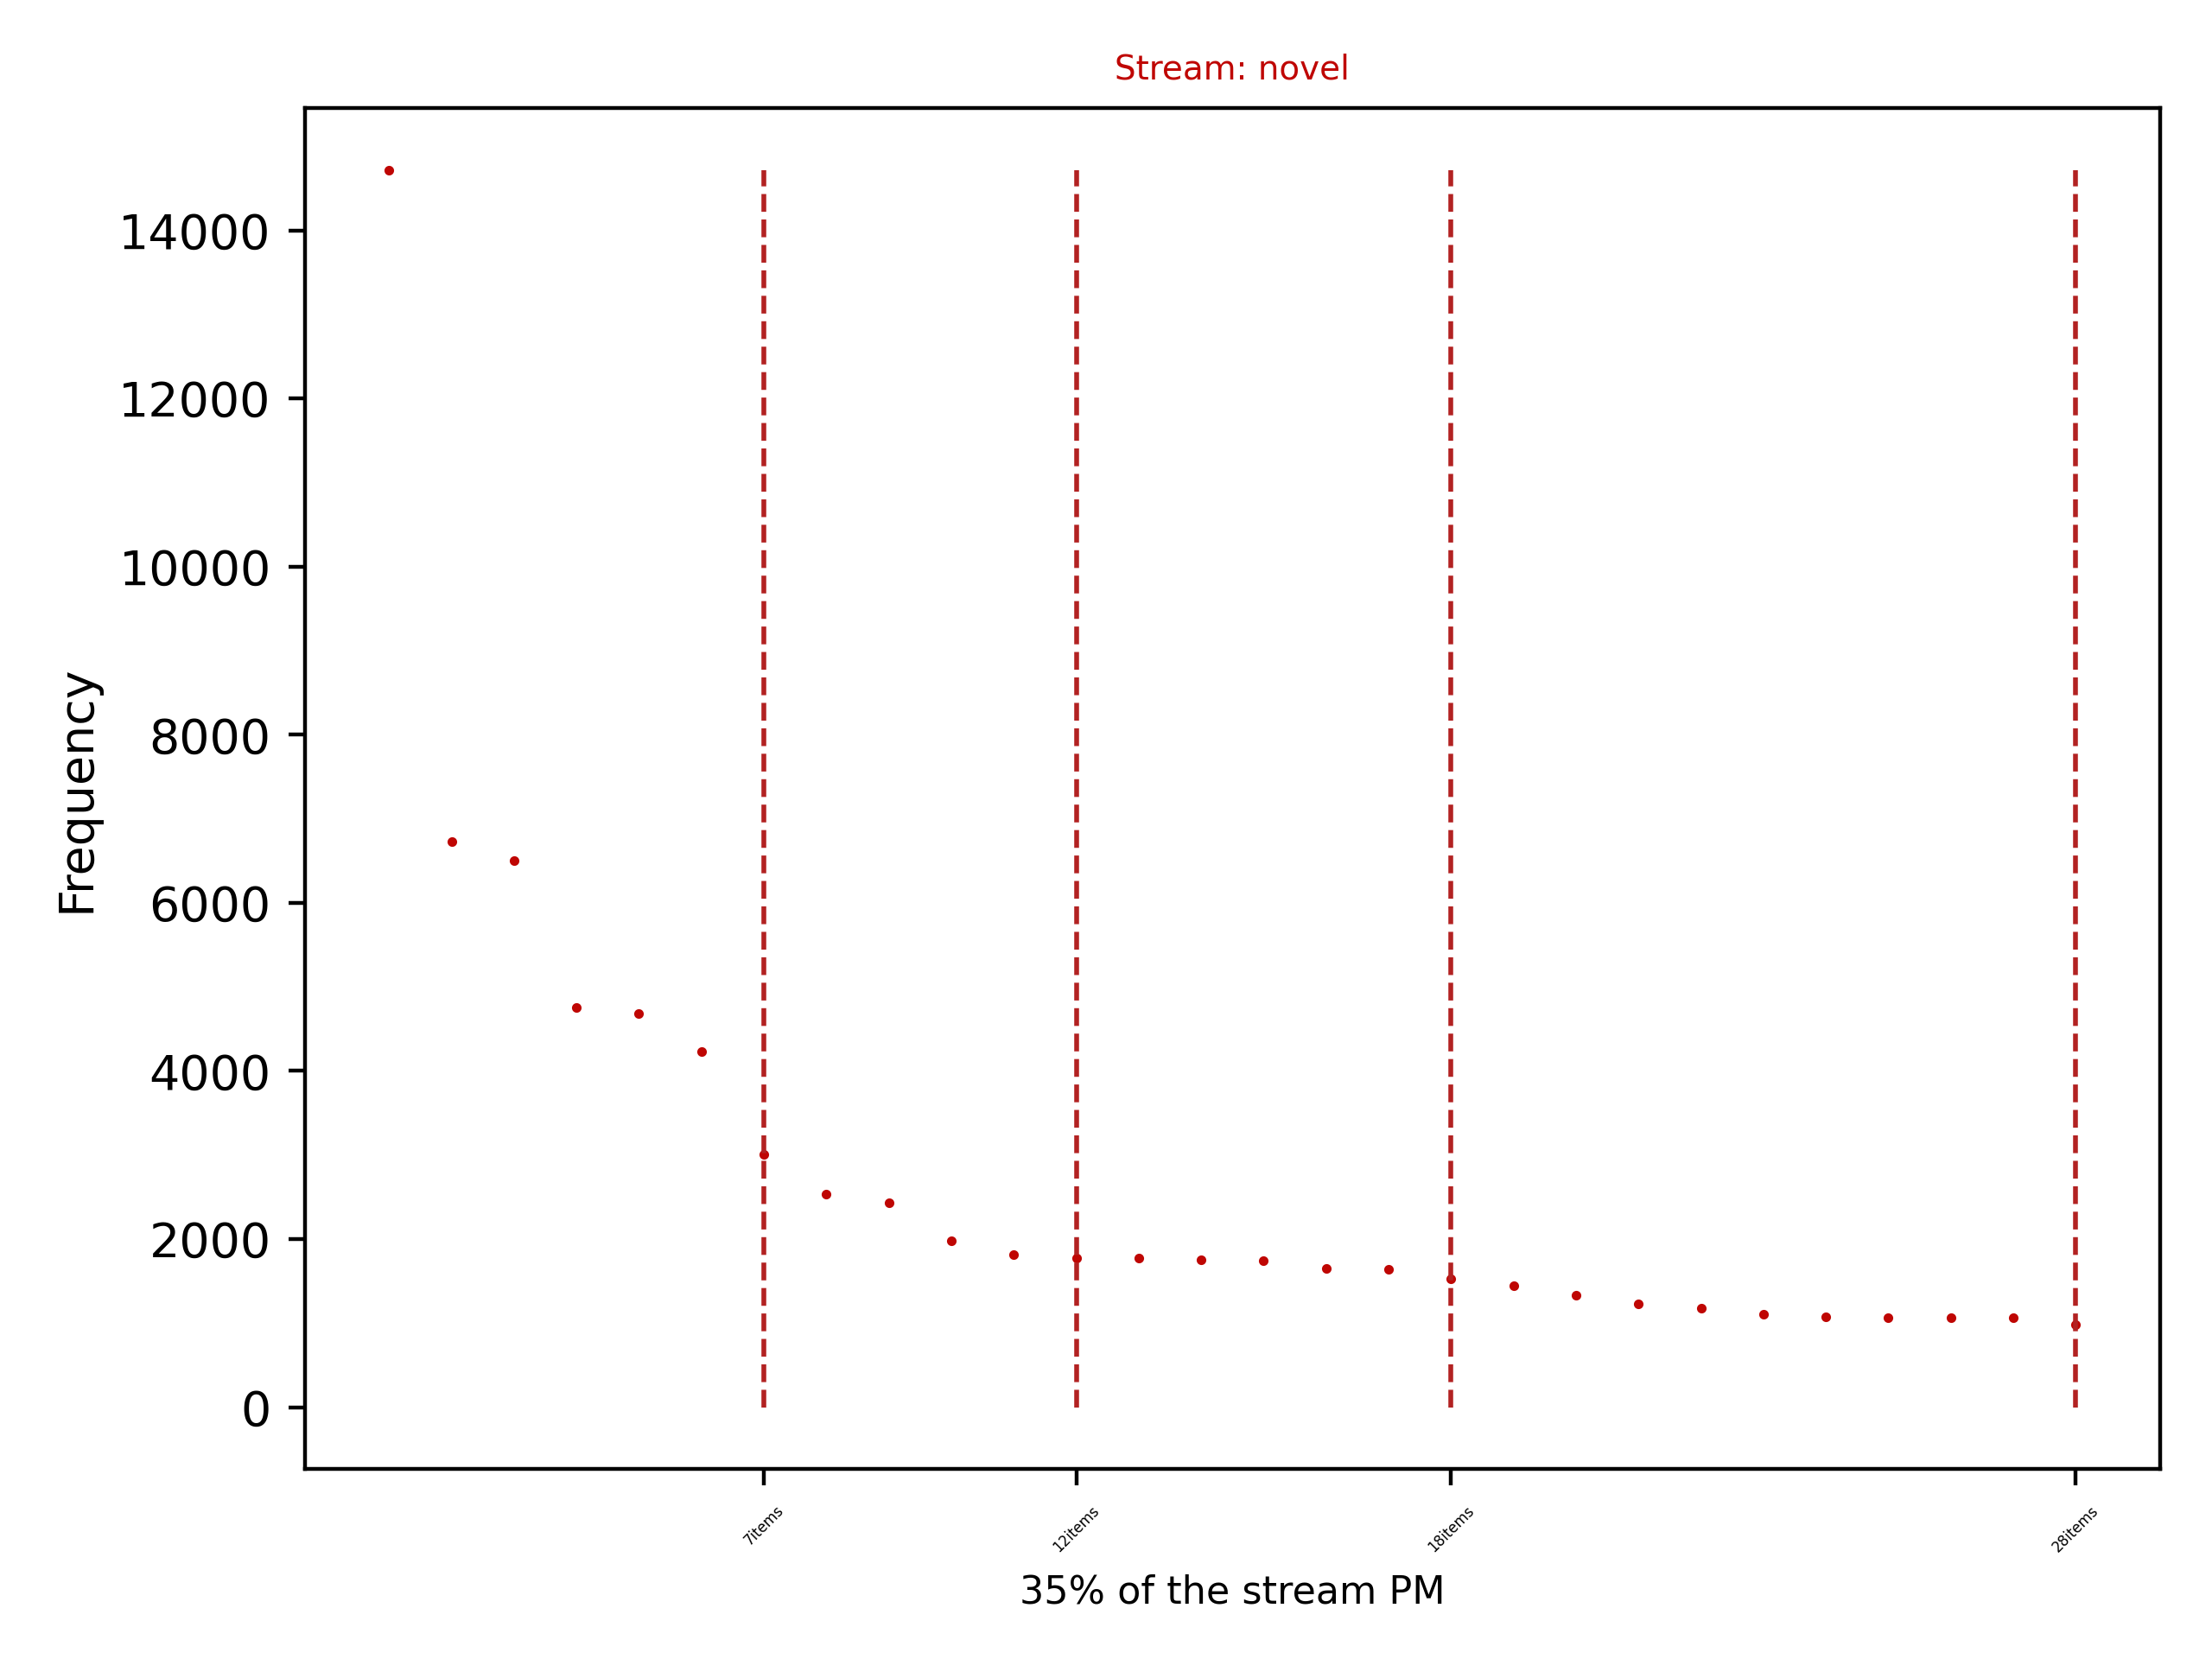
\includegraphics[width=\linewidth]{chapters/ch3_cfe/ch3_images/novel_pm.png}
    \caption*{Novel stream}
  \endminipage\hfill
  \minipage{0.32\textwidth}%
    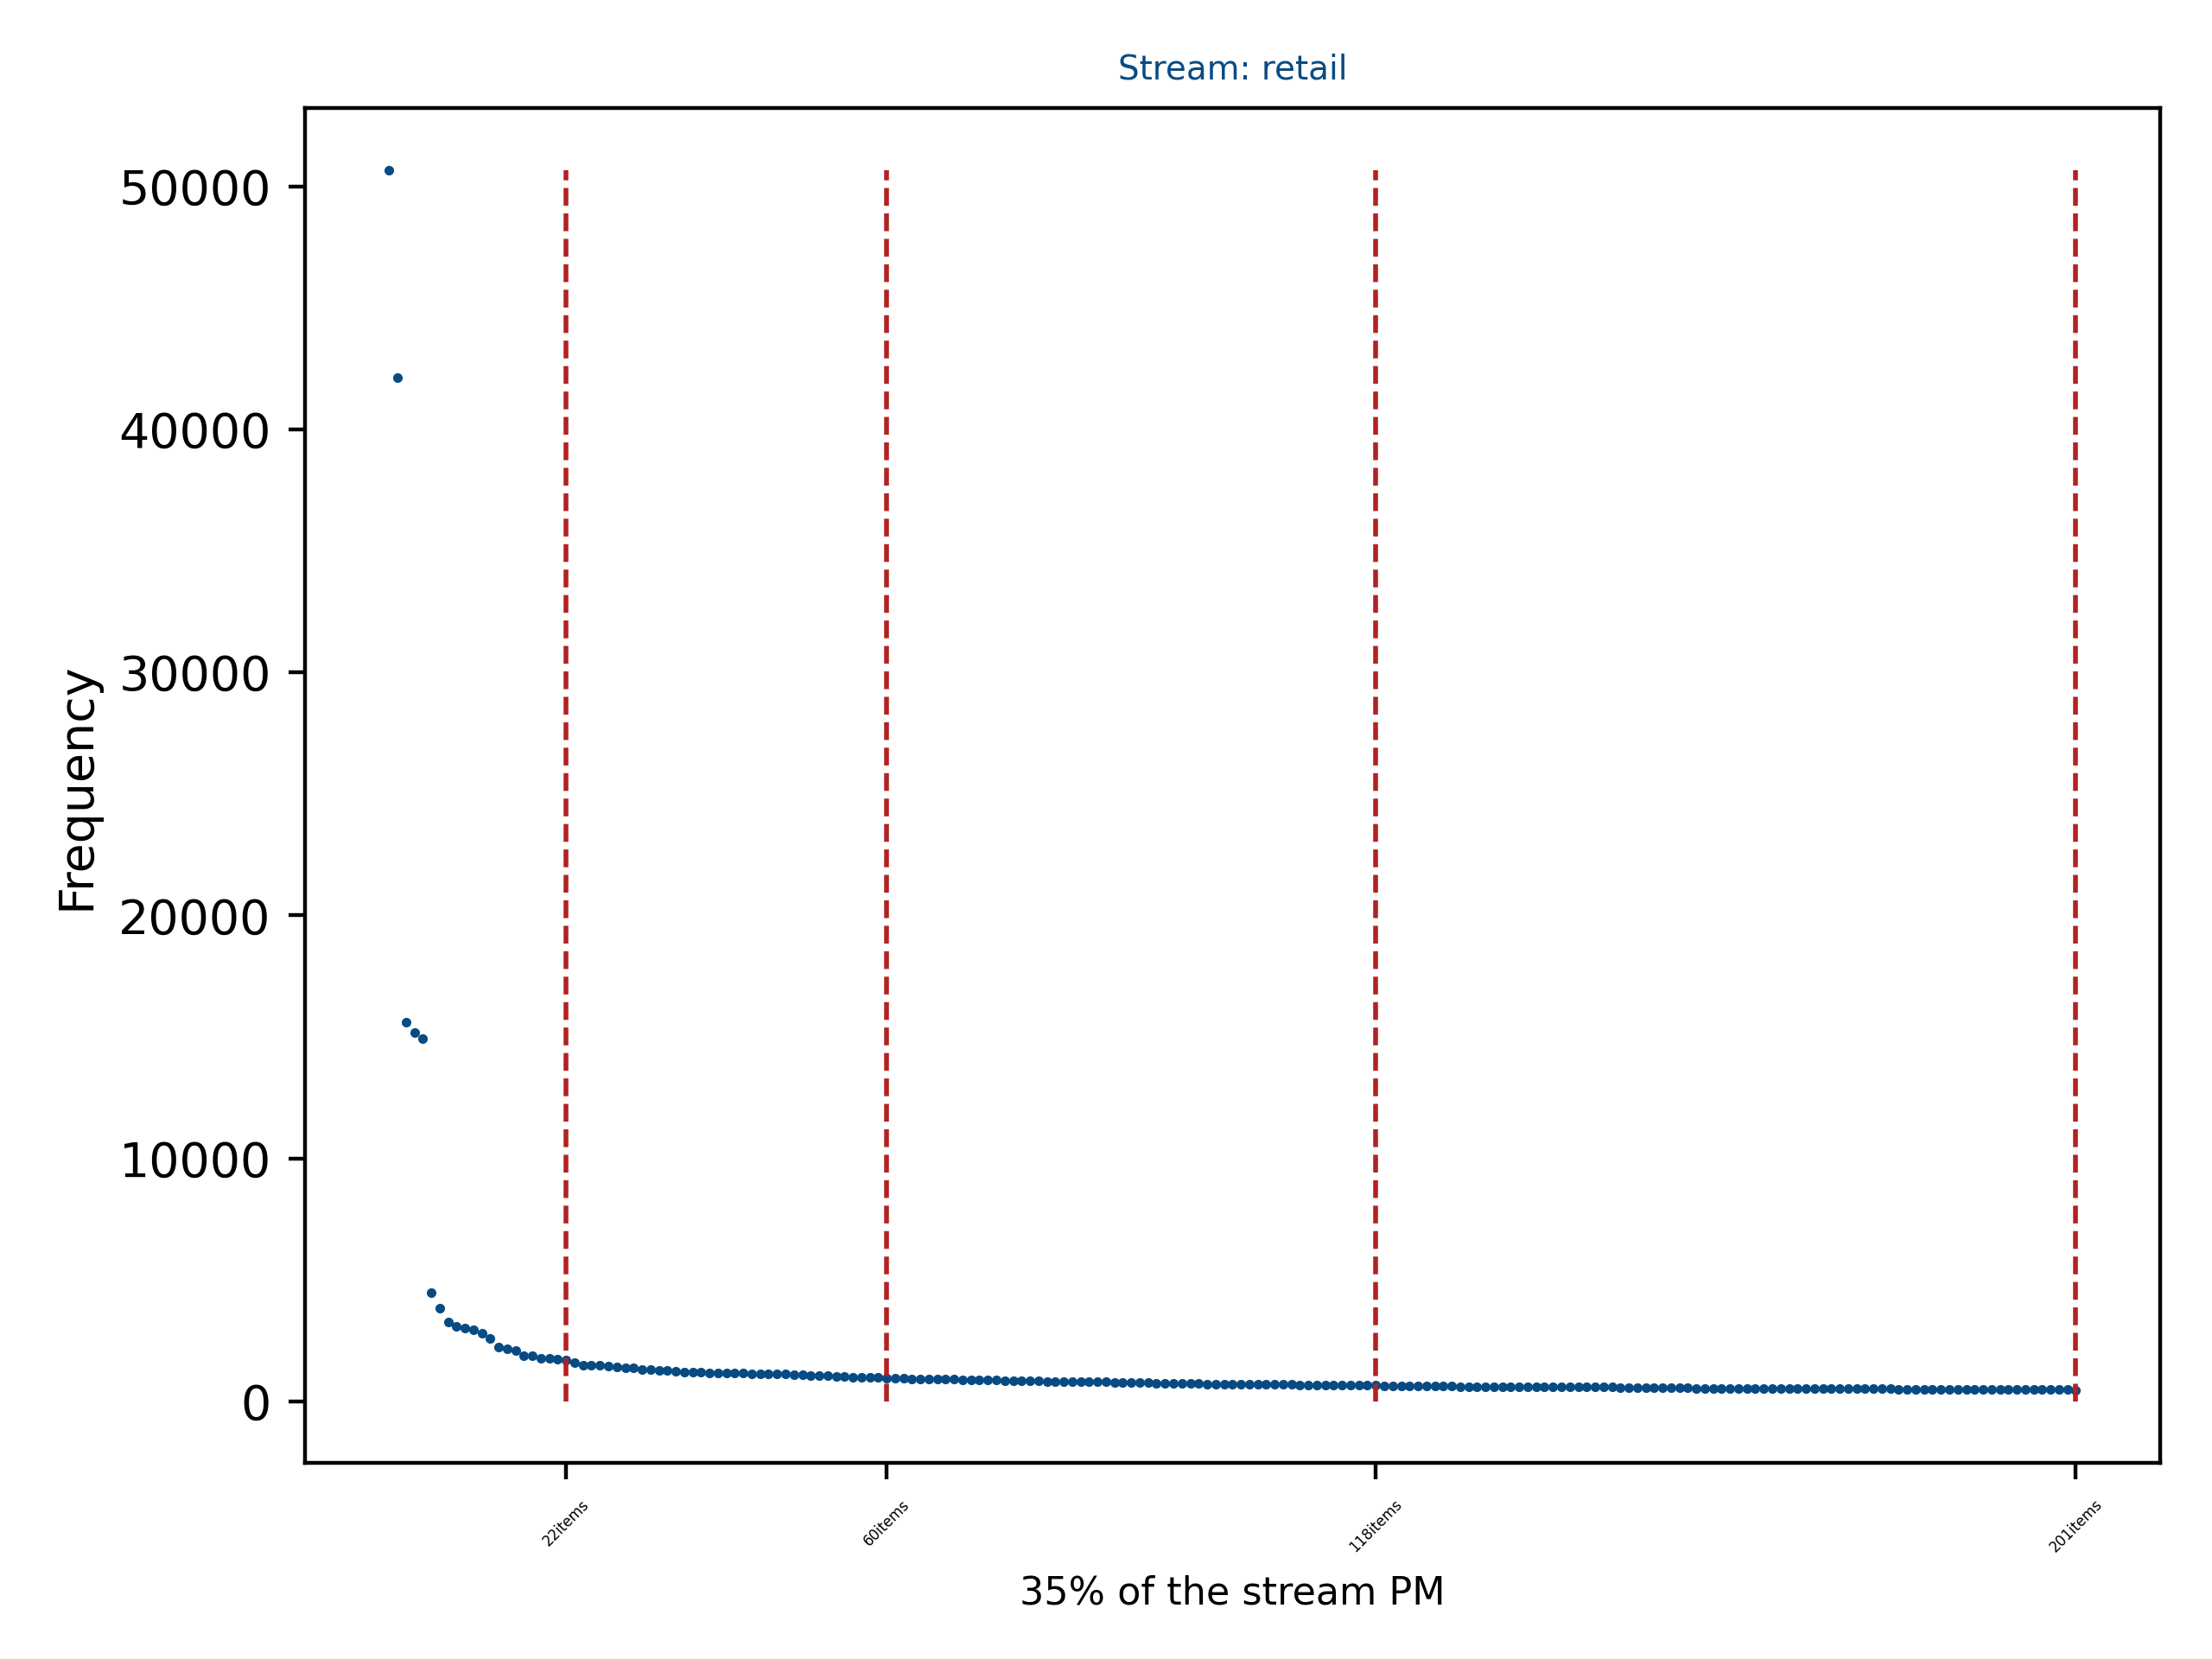
\includegraphics[width=\linewidth]{chapters/ch3_cfe/ch3_images/retail_pm.png}
    \caption*{Retail stream}
  \endminipage
  \caption[Stream Frequent Elements.]{We plot the top~$35\%$ probability mass for each stream. That is the most frequent elements that make up~$35\%$ of the total weight of the stream (i.e. the fewest number of elements in each stream whose frequencies sum to such that when divided by the total length of the stream equal~$35\%$). The first vertical red line in each plot is the top~$20\%$ probability mass, the second the top~$25\%$, the third the top~$30\%$, and the last the top~$35\%$. From visual inspection we decided to make the top-$K$ cut-off at, $20$ for Kosarak stream, $22$ for the Novel stream, and~$22$ for the Retail stream.}
  \label{fig:stream_pm} 
\end{figure*}
\paragraph{Measures and Metrics} We want to measure the performance of the CFEs of interest in the non-adversarial setting by determining how well they are able to identify and characterize the heavy elements in the streams above. %\mia{Why is it satisfactory to do it that way - aka test the streams only on limited number of streams? (if not addressed before)}

This problem, with varying but related definitions, is referred to in the literature as the heavy-hitters problem, the hot-items problem, or the top-$K$ problem. 

%\mia{[style] I think the sentence can be written better. 'to apply' - what do we actually mean by that? Can we be more concrete when giving the definition- possibly giving a bit more math-looking one as we have for some other stuff OR reference to a paper with it? }
The simplest of these definitions to apply is that of the top-$K$ problem, which is to simply report the set of elements with the~$K$ highest frequencies (for some~$K$) for a given stream. That is given elements of a stream~$\streamvar{S} \subseteq  \{ e_1,e_2,\ldots,e_M \}$ with associated frequencies~$(n_{e_1},n_{e_2},\ldots,n_{e_M})$ we can order the elements~$\{ e^{*}_{1},e^{*}_{2},\ldots,e^{*}_{M} \}$ such that~$(n^{*}_{e_1} \geq n^{*}_{e_2} \geq \ldots \geq n^{*}_{e_M})$. Then for some~$K \in \mathbb{Z}^{+}$ we output the set of elements~$\{ e^{*}_{1},e^{*}_{2},\ldots,e^{*}_{K} \}$ with the~$K$ highest frequencies~$(n^{*}_{e_1} \geq n^{*}_{e_2} \geq \ldots \geq n^{*}_{e_K})$.

The top-$K$ problem can be solved exactly given space linear to that of the stream by keeping an individual counter for each distinct element in the stream. It is not possible to solve exactly with space less than linear (see~\cite{Roughgarden_Valiant} for a formal impossibility argument), but it is a common technique to place a small data structure such as a min-heap restricted to size~$K$ on top of a CFE and by updating this small structure on each insertion once, one is able to approximate this top-$K$ set~\cite{yang2019heavykeeper,mandal2018topkapi,metwally2006}.

%\mia{How do we know this? Is it a common knowledge for CFE ppl - if so state it as such and give your source for the info.}. 

For our purposes we simply compute the approximate top-$K$ by processing the stream with a compact frequency estimator, querying on every distinct element in the stream, and ordering elements by approximated frequency. Likewise, we compute a true top-$K$ for each stream by processing said stream with a map linear in the size of the stream, computing a frequency for each element, and ordering by true frequency.  We note that we would have achieved identical results by putting a min-heap on top of each structure with fixed sized~$K$, updating as described in~\cite{yang2019heavykeeper} and outputting its contents once the entire stream has been processed. However, for experimental purposes our approach is more extensible than the one that would be used in practice.

%\mia{why don't we also consider the heap - this is possibly tom todo, why the alternative approach, what are its strengths (and weaknesses). How do we justify accepting the weaknesses?}

The number of heavy elements, or perhaps the number of heavy elements one would care about, varies depending on the stream and the application. For instance, it is noted that in a telecommunications scenario when monitoring the top outgoing call destinations of a customer typically a value of~$K$ in the range of~$10-20$ is appropriate~\cite{homen2010}. Moreover, when identifying the most frequent elements of interest of Zipfian distribution it is often of interest to vary~$K$ based on the parameters of the underlying distribution~\cite{charikar2002finding}.

We select~$K$ for each stream by observing the number of clearly identifiable outliers in the underlying stream.  We do this by visually inspecting the selected streams' frequency plots. We set the $x$-axis to enumerate all distinct elements in a stream, ordered from  most to least frequent and the $y$-axis as those distinct elements' corresponding frequencies. We make a cut-off around the point where the frequencies went from very peaked (distinct with prominent frequency jumps from element to element) to flat (many elements with about the same frequency -- the point at which the frequency differences decline less sharply). These frequency plots can be seen in Figure~\ref{fig:stream_pm}. We set~$K=20$ for the Kosarak stream,~$K=22$ for the novel stream, and~$K=22$ for the retail stream. 

We measure the accuracy of the non-adversarial performance according to four different metrics.

\begin{enumerate}
    \item \textbf{Set Intersection Size (SIS):} This measures the size of the set intersection of the true top-$K$ set~$\set{K}$ of the stream and the estimated top-$K$ set~$\tilde{\set{K}}$ as reported by the CFE:~$\text{SIS} = |\set{K} \cap \tilde{\set{K}}|$. This is measure of precision on the estimated top-$K$ set as compared to the true top-$K$ set. A SIS of~$K$ would imply perfect precision. 
    
    \item \textbf{Jaccard Index (JI):} The JI is a statistic that measures the similarity of two sets~\cite{real1996probabilistic}. We use the statistic to determine the similarity of the true top-$K$ set~$\set{K}$ of the stream and the estimated top-$K$ set~$\tilde{\set{K}}$ as reported by the CFE. It is defined as~$\mathrm{JI} = \frac{|\set{K} \cap \tilde{\set{K}}|}{|\set{K} \cup \tilde{\set{K}}|}$. A JI can be in the range~$[0,1]$, with a JI of~$1$ implying a perfect characterization of the true top-$K$ set by the CFE in its top-$K$ estimation. 
    
    \item \textbf{Minimal Top-$\tilde{K}$ to Capture True Top-K (MCT):} 
    This measures determines the minimal size~$L \geq K$ the estimated top-k set~$\tilde{\set{K}}$ would need to be to capture all elements contained in the true top-$K$ set~$\set{K}$. That is if one were to order the frequency estimates of all items made by a particular CFE, we would determine the number of items one would need to examine (starting from the most-frequent going down to the least-frequent) until all the elements from~$\set{K}$ were contained in that ordered set. Thus,~$L-K$ indicates the number of elements that fall out of~$\set{K}$ that are incorrectly being individually estimated to be greater than at least one element that is truly in~$\set{K}$. 
    
    \item \textbf{Average Relative Error on Top-k  elements (ARE)}:
    Average Relative Error is a standard measure to use when comparing CFEs~\cite{yang2019heavykeeper}. It is defined as~$\mathrm{ARE} = \frac{1}{K} \sum_{i=1}^{K} \frac{| \hat{n_{i}} - n_{i}|}{n_{i}}$
    where $i \in [K]$ indexes the true top-$K$ elements for a particular stream.
\end{enumerate}

\paragraph{Results} We crafted reference implementations for all three CFEs of interest: CMS, HK, and CK\footnote{Source code is available at: \url{https://github.com/smarky7CD/cfe-in-adv-envs}}. They are implemented in Python3 and use the BLAKE2b cryptographic hash function %(a 64-bit output hash) 
for independent row hash functions and for a fingerprint hash function in the case of CK and HK. %\mia{How big are fps and cnts? Or is it a parameter that a person running our implementation can vary?} \smnote{Technically, unbounded due to Python, but all remain under 32 bits in size in practice .}

We are interested in comparing performance when the space used by the structures is held constant. Observe that CK is three times as large as  CMS, and HK is twice as large as CMS assuming the same space is used for a counter bucket and a fingerprint bucket (in the CK and HK) across all structures. In practice these buckets could be (say)~$32$-bits. We picked two sets of parameters, a \emph{standard} set and a \emph{constrained} set to test.

The standard set of parameters set~$m=2048,k=4$ for CMS,~$m=1024,k=4$ for HK, and~$m=910,k=3$ for CK. This corresponds to~$32.76$~kB of space when using a 32-bit bucket sizes. We experimentally show that at this size all the structures are able to identify the heavy elements of the streams we test upon with minimal to no error. 

The constrained set of parameters sets~$m=512,k=4$ for CMS,~$m=256,k=4$ for HK, and~$m=341,k=2$ for CK. This corresponds to just~$8.19$~kB of space when using a 32-bit counter and fingerprint bucket sizes. In this space constrained setting the structures are still able to identify the heavy elements of the streams we test upon, but with some degree of moderate error. 

For HK, we set~$d=0.9$ for all experiments, as this is the default chosen by Redis~\cite{redisbloom} and satisfies the desired properties of the exponential decay function stated in~\cite{yang2019heavykeeper}. 

We ran~$1000$ trials for each structure, stream, and parameter triplet using our reference implementations. We randomize each trial on the particular choice of hash functions used for the rows (by selecting a random per-trial seed), as well as the order in which the items in the stream are processed. The latter simulates an item being randomly drawn from the underlying distribution of the stream. We averaged our four metrics for each structure, stream and parameter triplet over the~$1000$ trials. 

\begin{table*}[!ht]
  \centering
  \begin{tabular}{|ccccccc|}
  \hline
  \multicolumn{1}{|c|}{\textbf{Structure}} & \multicolumn{1}{c|}{\textbf{\begin{tabular}[c]{@{}c@{}}Parameters\\ (m,k)\end{tabular}}} & \multicolumn{1}{c|}{\textbf{Stream}}                                                                   & \multicolumn{1}{c|}{\textbf{SIS}}                                                     & \multicolumn{1}{c|}{\textbf{JI}}                                                   & \multicolumn{1}{c|}{\textbf{MCT}}                                                      & \textbf{ARE}                                                  \\ \hline
  \multicolumn{7}{|l|}{\textit{Standard}}                                                                                                                                                                                                                                                                                                                                                                                                                                                                                                                                               \\ \hline
  \multicolumn{1}{|c|}{CK}                 & \multicolumn{1}{c|}{(910,3)}                                                             & \multicolumn{1}{c|}{\multirow{3}{*}{\begin{tabular}[c]{@{}c@{}}Kosarak~($K=20$)\\ Novel~($K=22$)\\ Retail~($K=22$)\end{tabular}}} & \multicolumn{1}{c|}{\begin{tabular}[c]{@{}c@{}}20\\ 22\\ 22\end{tabular}}             & \multicolumn{1}{c|}{\begin{tabular}[c]{@{}c@{}}1\\ 1\\ 1\end{tabular}}             & \multicolumn{1}{r|}{\begin{tabular}[c]{@{}r@{}}20\\ 22\\ 22\end{tabular}}              & \begin{tabular}[c]{@{}c@{}}$\approx 0$\\ $\approx 0$\\ $\approx 0$\end{tabular}             \\ \cline{1-2} \cline{4-7} 
  \multicolumn{1}{|c|}{CMS}                & \multicolumn{1}{c|}{(2048,4)}                                                            & \multicolumn{1}{c|}{}                                                                                  & \multicolumn{1}{c|}{\begin{tabular}[c]{@{}c@{}}19.303\\ 22.999\\ 21.643\end{tabular}} & \multicolumn{1}{c|}{\begin{tabular}[c]{@{}c@{}}0.934\\ 0.999\\ 0.997\end{tabular}} & \multicolumn{1}{r|}{\begin{tabular}[c]{@{}r@{}}20.901\\ 22.001\\ 22.405\end{tabular}}  & \begin{tabular}[c]{@{}c@{}}0.017\\ 0.009\\ 0.040\end{tabular} \\ \cline{1-2} \cline{4-7} 
  \multicolumn{1}{|c|}{HK}                 & \multicolumn{1}{c|}{(1024,4)}                                                            & \multicolumn{1}{c|}{}                                                                                  & \multicolumn{1}{c|}{\begin{tabular}[c]{@{}c@{}}20\\ 22\\ 22\end{tabular}}             & \multicolumn{1}{c|}{\begin{tabular}[c]{@{}c@{}}1\\ 1\\ 1\end{tabular}}             & \multicolumn{1}{r|}{\begin{tabular}[c]{@{}r@{}}20\\ 22\\ 22\end{tabular}}              & \begin{tabular}[c]{@{}c@{}}$\approx 0$\\ $\approx 0$\\ $\approx 0$\end{tabular}             \\ \hline
  \multicolumn{7}{|l|}{\textit{Constrained}}                                                                                                                                                                                                                                                                                                                                                                                                                                                                                                                                               \\ \hline
  \multicolumn{1}{|c|}{CK}                 & \multicolumn{1}{c|}{(341,2)}                                                             & \multicolumn{1}{c|}{\multirow{3}{*}{\begin{tabular}[c]{@{}c@{}}Kosarak~($K=20$)\\ Novel~($K=22$)\\ Retail~($K=22$)\end{tabular}}} & \multicolumn{1}{c|}{\begin{tabular}[c]{@{}c@{}}17.189\\ 21.617\\ 13.442\end{tabular}} & \multicolumn{1}{c|}{\begin{tabular}[c]{@{}c@{}}0.757\\ 0.967\\ 0.441\end{tabular}} & \multicolumn{1}{c|}{\begin{tabular}[c]{@{}c@{}}28.695\\ 22.451\\ 209.439\end{tabular}} & \begin{tabular}[c]{@{}c@{}}$\approx 0$\\ $\approx 0$\\ 0.021\end{tabular}         \\ \cline{1-2} \cline{4-7} 
  \multicolumn{1}{|c|}{CMS}                & \multicolumn{1}{c|}{(512,4)}                                                             & \multicolumn{1}{c|}{}                                                                                  & \multicolumn{1}{c|}{\begin{tabular}[c]{@{}c@{}}18.241\\ 21.638\\ 18.745\end{tabular}} & \multicolumn{1}{c|}{\begin{tabular}[c]{@{}c@{}}0.841\\ 0.969\\ 0.745\end{tabular}} & \multicolumn{1}{c|}{\begin{tabular}[c]{@{}c@{}}24.567\\ 22.473\\ 41.609\end{tabular}}  & \begin{tabular}[c]{@{}c@{}}0.125\\ 0.062\\ 0.296\end{tabular} \\ \cline{1-2} \cline{4-7} 
  \multicolumn{1}{|c|}{HK}                 & \multicolumn{1}{c|}{(256,4)}                                                             & \multicolumn{1}{c|}{}                                                                                  & \multicolumn{1}{c|}{\begin{tabular}[c]{@{}c@{}}20\\ 22\\ 21.976\end{tabular}}         & \multicolumn{1}{c|}{\begin{tabular}[c]{@{}c@{}}1\\ 1\\ 0.998\end{tabular}}         & \multicolumn{1}{c|}{\begin{tabular}[c]{@{}c@{}}20\\ 22\\ 55.008\end{tabular}}          & \begin{tabular}[c]{@{}c@{}} $\approx 0$\\ 0.001\\ 0.005\end{tabular}     \\ \hline
  \end{tabular}
  \caption[Non-adversarial CFE Results.]{A summary of non-adversarial setting results between the CK, CMS, and HK compact frequency estimators.}
  \label{tab:hon-exp-res}
  \end{table*}


We present a summary of the results in Table~\ref{tab:hon-exp-res}. For the \emph{standard} parameter set we see that CK and HK perform best, being able to perfectly capture the true top-$K$ set for each stream with their outputted estimated top-$K$ set in \emph{every} trial. This is indicated by the SIS and MCT being equal to~$K$ and the JI being equal to~$1$ for each stream. Moreover, the estimates on these top-$K$ elements for both of these structures were very tight. The ARE over all trials and streams was~$0$ (ignoring a small rounding error). This indicates that CK and HK nearly perfectly individually estimated every single element in the true top-$K$ across all trials. 
  
CMS with the standard parameter sizing performs almost as well. Only failing to capture the true top-$K$ set with its estimated set a few number of times over the~$1000$ trials. This is indicated by the SIS and MCT being very close to~$K$ and the JI being very close to~$1$ for each stream. However, CMS, as it is prone to overestimation on every element, has slightly higher ARE than the other structures. 

The \emph{constrained} set of parameters presents a challenge for all the CFEs in computing individual frequency estimations on elements in the streams, and as a result computing an accurate estimated top-$K$. This setting only allocates CK a measly~$642$ individual counters to compactly represent streams that all have over~$19,000$ distinct elements. Under these conditions, HK performs best according to our metrics. It perfectly captures the true top-$K$ in both the Kosarak and Novel stream, while only failing to do so in a handful of trials with the Retail stream. Moreover, the ARE is small across all streams -- comparatively less than CMS with the standard parameters. HK by design prioritizes providing accurate estimates on the most frequent elements, by way of its probabilistic decay mechanism. So while it performs well on this task, it severely underestimates middling and low frequency elements at this sizing, reporting an individual frequency estimate very near~$0$ for any element that is not heavy. %This behavior is what we exploit in our attacks to create error in the structure, effectively masking true heavy elements. 

 CMS and CK perform less well in this small space allocation setting. While CMS performs slightly better in capturing the true top-$K$ set within its estimated top-$K$ set, CK continues to give better accuracy on individual point estimations of the true top-$K$ elements across streams due to its internal sub-estimators that provide tighter estimations than CMS.

We observe in this constrained space setting across the structures measured performance is the worst on the Retail stream. This is because the Retail stream has a flatter distribution as compared to the other streams. That is to say, it has very few clearly identifiable heavy elements before containing a large collection of elements of about the same frequency. This can be seen in the frequency plot in Figure~\ref{fig:stream_pm}. The Retail element with frequency rank~$22$ has a true frequency of~$1715$ while the Retail element of frequency rank~$56$ has a true frequency of~$1005$. Comparing this to $n_{22} = 22631, n_{56} = 9559$ and~$n_{22} = 1176, n_{56} = 474$, respectively for the Kosarak and Novel stream, one can see that the relative fall off in true frequency is far less pronounced within this region of the Retail stream. This in turn leads to small errors in the individual frequency estimations of elements near (but outside) the true top-$K$ of the Retail stream propagating to the top-$K$ estimation -- by making it challenging for the CFEs to draw a clear distinction between the truly heavy elements and the nearly heavy elements. The upshot being, one needs larger structures to accurately estimate these flatter streams.

In sum, CK performs comparatively well to both CMS and HK in this particular task. In fact, CK performed better than CMS when not burdened with \emph{very} tiny space constraints. It is able to perfectly estimate the true top-$K$ for all streams over all trials with only $2730$ individual counters in the standard parameter setting, while also being adversarial robust where the others structures are not. 

